\begin{frame}{Нелинейное уравнение Шрёдингера}
		\begin{tcolorbox}[
		colframe=DeepBlue!35, 
		colback=DeepBlue!1!Ivory, 
		boxrule=0.5pt, arc=3pt, 
		top=4pt, bottom=4pt, left=4pt, right=4pt,
		before=\vspace{6pt}, after=\vspace{0pt} % Увеличен отступ от заголовка (before)
		]
			\[
			\begin{cases}
				iu_t+au_{xx} + bu_{yy}+c|u|^2u + du = 0 \\
				u(x, y, 0) = u_0(x, y)
			\end{cases}
			\]
		\end{tcolorbox}
	\begin{figure}
		\centering
		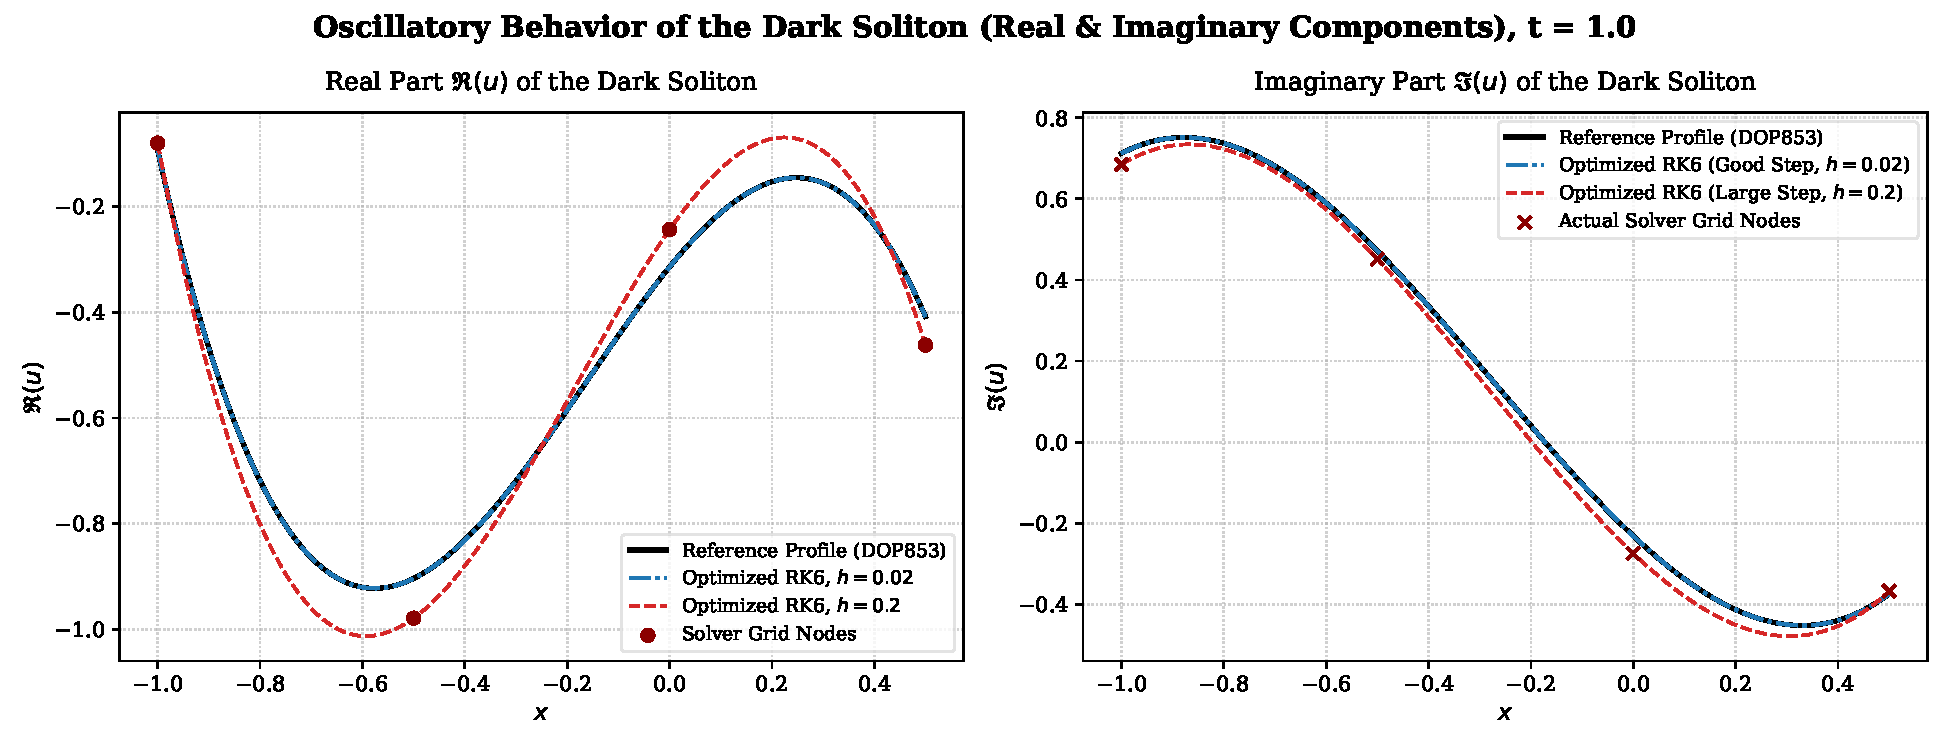
\includegraphics[width=\linewidth]
		{../code/results/visualization/nls_components_visualized}
	\end{figure}
	
\end{frame}